\documentclass[pdftex,12pt,xcolor=svgnames]{beamer}

\mode<presentation>
{
  \usetheme{boxes}
  \usecolortheme[named=MidnightBlue]{structure}
  %\setbeamercolor{normal text}{bg=NavajoWhite!20}
  \usefonttheme{serif}
  \setbeamertemplate{navigation symbols}{}
  % Show frame number and author name in footline
  \setbeamertemplate{footline}[frame number]
  \addtobeamertemplate{footline}{\quad\textcolor{gray}{James Robert Lloyd}}{}
  % Set frame titles in small capitals
  \setbeamerfont{frametitle}{shape=\scshape,family=\rmfamily}
  \setbeamercolor{frametitle}{bg=gray!60!white,fg=black}
  % Alerted text: blue (uncomment second line if theme sets alerted text to bold)
  \setbeamercolor{alerted text}{fg=blue}
  %\setbeamerfont*{alerted text}{}
  \setbeamertemplate{bibliography item}[text] %{\hbox{\donotcoloroutermaths$\blacktriangleright$}}
  \setbeamertemplate{bibliography entry title}{}
  \setbeamertemplate{bibliography entry author}{}
  \setbeamertemplate{bibliography entry note}{}
  \setbeamertemplate{bibliography entry location}{}

}
\usepackage[english]{babel}
\usepackage[latin1]{inputenc}
\usepackage{times}
\usepackage[T1]{fontenc}
\usepackage{hyperref}
\usepackage{multimedia}
\usepackage{eepic}
\usepackage{graphicx}
%\usepackage[nohug]{latexinclude/diagrams}
\usepackage{tikz}
\usetikzlibrary{calc}

%% \newcommand{\footlineextra}[1]{
%%     \begin{tikzpicture}[remember picture,overlay]
%%         \node[yshift=1.5ex,anchor=south east] at (current page.south east)
%% {#1};
%%     \end{tikzpicture}
%% }

\newcommand{\footlineextra}[1]{
    \begin{tikzpicture}[remember picture,overlay]
        \node[xshift=-5ex,yshift=-0.5ex,anchor=south east] at (current page.south east)
             {\mbox{\tiny \textcolor{MidnightBlue}{#1}}};
    \end{tikzpicture}
}

\def\sectionframe#1{
  {
    \setbeamertemplate{footline}{\empty}
    \begin{frame}{}
      \begin{center}
        \huge\sc #1
      \end{center}
    \end{frame}
  }
}


\usepackage{etex}

\usepackage{tabularx}
\usepackage{include/picins}
\usepackage{include/preamble}
\usepackage{tikz}

\usetikzlibrary{shapes.geometric,arrows,chains,matrix,positioning,scopes,calc}

%%%%%%%%%%%%%%%%%%%%%%%%%%%%%%%%%%%%%%%%%%%
%
% Some look and feel definitions
%
%%%%%%%%%%%%%%%%%%%%%%%%%%%%%%%%%%%%%%%%%%%

\setlength{\columnsep}{0.03\textwidth}
\setlength{\columnseprule}{0.0018\textwidth}
\setlength{\parindent}{0.0cm}

\tikzstyle{mybox} = [draw=white, rectangle]

\definecolor{camlightblue}{rgb}{0.601 , 0.8, 1}
\definecolor{camdarkblue}{rgb}{0, 0.203, 0.402}
\definecolor{camred}{rgb}{1, 0.203, 0}
\definecolor{camyellow}{rgb}{1, 0.8, 0}
\definecolor{lightblue}{rgb}{0, 0, 0.80}
\definecolor{white}{rgb}{1, 1, 1}
\definecolor{whiteblue}{rgb}{0.80, 0.80, 1}

\newcolumntype{x}[1]{>{\centering\arraybackslash\hspace{0pt}}m{#1}}
\newcommand{\tabbox}[1]{#1}

\hypersetup{colorlinks=true,citecolor=blue}

%%%%%%%%%%%%%%%%%%%%%%%%%%%%%%%%%%%%%%%%%%%
%
% The talk
%
%%%%%%%%%%%%%%%%%%%%%%%%%%%%%%%%%%%%%%%%%%%

\title{Building an automatic statistician}

\author{
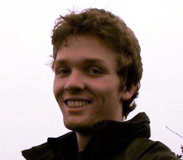
\includegraphics[height=0.2\textwidth]{figures/JamesLloyd4}
\qquad
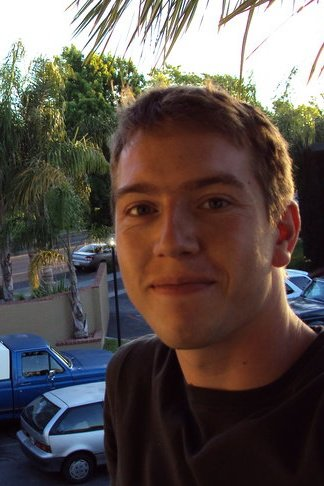
\includegraphics[height=0.2\textwidth, trim=20mm 25mm 0mm 25mm, clip]{figures/david2}
\qquad
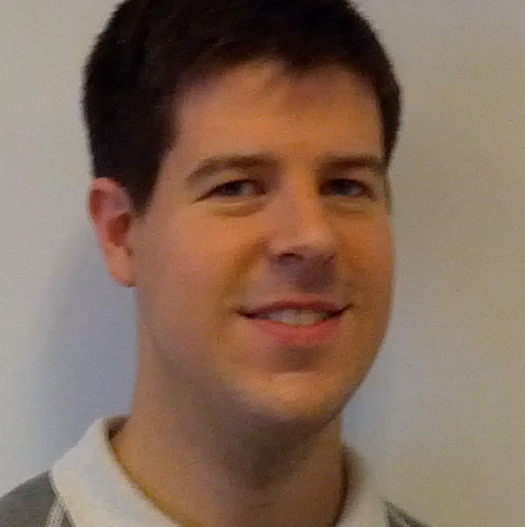
\includegraphics[height=0.2\textwidth]{figures/roger-photo}
\\
James Robert Lloyd, David Duvenaud, Roger Grosse,\\
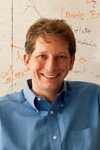
\includegraphics[height=0.2\textwidth, trim=0mm 7mm 0mm 0mm, clip]{figures/josh2}
\qquad
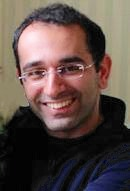
\includegraphics[height=0.2\textwidth]{figures/zg2}\\
Joshua Tenenbaum, Zoubin Ghahramani
}

\begin{document}

\frame[plain] {
\titlepage
}

\begin{frame}{There is a growing need for data scientists}
  \begin{itemize}
    \item Abundant data
    \vspace{\baselineskip}
    \item McKinsey Global Institute quotation
    \vspace{\baselineskip}
    \item Automating this process would have a tremendous impact on various fields
    \begin{itemize}
       \item Computational biology
       \item Stuff
     \end{itemize}
  \end{itemize}
\end{frame}

\begin{frame}{Prerequisites for an automatic statistician}
  \begin{itemize}
    \item An open-ended language of models
    \begin{itemize}
       \item Content
       \item Content
     \end{itemize}
    \vspace{\baselineskip}
    \item A search procedure
    \vspace{\baselineskip}
    \item A principled method of evaluating models
    \vspace{\baselineskip}
    \item A procedure to automatically explain the models
  \end{itemize}
\end{frame}

\begin{frame}{Defining a language of regression models}
  \begin{itemize}
    \item $f: \mathcal{X} \to \mathcal{Y}$
    \vspace{\baselineskip}
    \item Want to represent simple parametric forms
    \begin{itemize}
       \item Linear functions
       \item Polynomials
       \item Exponential functions \ldots
     \end{itemize}
    \vspace{\baselineskip}
    \item Also want to represent complex nonparametric functions specified in terms of high level proper ties
    \begin{itemize}
       \item Smoothness
       \item Periodicity \ldots
     \end{itemize}
  \end{itemize}
\end{frame}

\begin{frame}{We can do this with Gaussian processes}
  \begin{itemize}
    \item Definition
    \vspace{\baselineskip}
    \item Completely specified by mean and covariance
    \vspace{\baselineskip}
    \item We can integrate out the mean in many situations
    \vspace{\baselineskip}
    \item So let's focus on the covariance / kernel
  \end{itemize}
\end{frame}

\begin{frame}{The atoms of the language}
  Show pictures of different function types from base kernels
\end{frame}

\begin{frame}{The composition rules of our language}
  Addition and multiplication with pictures
\end{frame}

\begin{frame}{Modelling changepoints}
  Addition and multiplication with pictures
\end{frame}

\begin{frame}{An expressive language of models}
  Table
\end{frame}

\begin{frame}{Exploring the language}
  \begin{itemize}
    \item Large and open ended
    \vspace{\baselineskip}
    \item Need to be efficient
    \vspace{\baselineskip}
    \item Try to mimick human behaviour
  \end{itemize}
\end{frame}

\begin{frame}{A greedy search}
  Make a new example of kernel learning
\end{frame}

\begin{frame}{Model evaluation}
  Need to trade off complexity and model fit
  
  Bayesian Occam's razor
  
  Multiple slides on this
\end{frame}

\begin{frame}{How can we describe a model}
  Motivating example of $\kSE \times \kPer \times \kLin$.
\end{frame}

\begin{frame}{How can we describe a model}
  Show a big expression
\end{frame}

\begin{frame}{How can we describe a model}
  Convert changepoint operator
\end{frame}

\begin{frame}{How can we describe a model}
  Distributes sums over products
\end{frame}

\begin{frame}{How can we describe a model}
  Sums of kernels are sums of products - maths and picture
\end{frame}

\begin{frame}{How can we describe a model}
  Show the build up of an $\kSE \times \kPer \times \kLin \times \boldsymbol\sigma$ kernel starting with the noun and adding modifiers
  
  Then show the underset kernel description
\end{frame}

\begin{frame}{Example: Airline}
\end{frame}

\begin{frame}{Example: Solar}
\end{frame}

\begin{frame}{Example: Call centre}
\end{frame}

\begin{frame}{Example: Sulphuric}
\end{frame}

\begin{frame}{Good predictive performance as well}
  Interpretability / accuracy trade-off rears its annoying head - but both are pretty good :)
\end{frame}

\begin{frame}{Challenges}
  
\end{frame}

\begin{frame}{Current and future directions}
  
\end{frame}

\begin{frame}{Summary}
  
\end{frame}

\end{document}

\begin{frame}{Title}
  \begin{itemize}
    \item Content
    \vspace{\baselineskip}
    \item Content
    \vspace{\baselineskip}
    \item Content
    \begin{itemize}
       \item Content
       \item Content
     \end{itemize}
  \end{itemize}
\end{frame}